\chapter{Background}
When a human first plays a game, let it be chess, poker, Minecraft, CS:GO or any other game, it is not given any instructions on how to play. It is not told which moves are good and which are bad, maybe it doesn't even know the rules of the game. By interacting and playing the game, losing to some opponents and starting to beat others, the player gradually learns what moves are best in which situation and starts to understand the dynamics of the game. During all of this the player doesn't have any external feedback telling him which actions to perform in a given situation, but has to learn it by itself, by performing an action and experiencing the outcome. Learning from interaction is a foundational idea underlying nearly all theories of learning and intelligence \cite{sutton-barto}.\\\\
In this chapter we provide an overview of reinforcement learning. First we will discuss Markov Decision Processes (MDPs) that allow us to define an environment (for now we can think of an environment as a game) in mathematical terms, then we will discuss Dynamic Programming, that allows to solve exactly the reinforcement learning problem in case we know everything about the environment. Finally, we will see model-free methods, that allow us to learn even if we know nothing about the environment, these methods learn by interacting directly with the environment, obtaining experience and exploiting it to find the best actions to perform in any situation. This chapter is based on the first part of the Sutton and Barto book \cite{sutton-barto}

\section{Reinforcement Learning}
Reinforcement learning is the field of machine learning that tries to maximize a numerical reward signal. The agent is not said which actions to take, but instead must discover the actions that lead to the highest reward by trying them. Furthermore, actions do not only influence the immediate future reward but also the next situation and consequently subsequent rewards, so the agent must learn to balance immediate and future rewards.\\\\
Reinforcement learning differs from supervised learning because there is no external supervisor, which tells the agent which actions to perform in a given situation, instead the agent must discover the actions that lead to the highest reward by trying them. 
Reinforcement learning is also different from unsupervised learning, because even though both approaches do not need labels to learn from, their goal is different. In unsupervised learning the goal is to find structure in the data, while in reinforcement learning the goal is to maximize a reward signal.\\\\
One important aspect of reinforcement learning is the exploration-exploitation trade-off, which is not present in supervised or unsupervised learning. The agent must weigh the benefits of exploring new actions against the benefits of utilizing the best actions it has already discovered. A focus on exploration alone may lead to the discovery of the best actions, but with infrequent use, while a focus on exploitation alone may prevent the discovery of potentially better actions.

\section{Markov Decision Processes}
We can formalize the problem of learning from interaction to achieve a goal with Markov Decision Processes (MDPs). In the MPD framework the learner is called the agent, and the thing it interacts with is called the environment. The agent continually interacts with the environment by performing actions, on each action the environment changes state, and presents a new situation to the agent. The environment is also responsible to give the reward signal the agent must maximize \ref{fig:mdp}.
\begin{figure}[H]
    \centering
    \includesvg[width=0.6\textwidth]{images/mdp.svg}
    \caption{Illustration of the agent-environment interaction in a Markov Decision Process}
    \label{fig:mdp}
\end{figure}
More specifically, the agent and environment interact in discrete time steps ($t=0, 1, 2 \dots$). At each time step $t$ the agent receives an observation of the environment's state $S_t \in S$ and based on that chooses an action $A_t \in A$. In the next time step $t+1$ the agent receives from the environment a numerical reward $R_{t+1} \in R \in \mathbb{R}$ and a new observation $S_{t+1} \in S$ and so on. This generates a sequence of observations, actions and rewards, which we call trajectory: $S_0, A_0, R_1, S_1, A_1, R_2, \dots$.\\\\
In finite MDPs the set of states $S$, actions $A$ and rewards $R$ are finite, so the distribution of next state and reward, given the current state and action is well defined. Furthermore, the distribution of the random variables $R_t$ and $S_t$ follows the Markov property, depending only on the previous state and action, $P(S_{t+1}|S_t) = P(S_{t+1}|S_t, S_{t-1}, \dots, S_0)$.\\\\
We can formalize mathematically an MDP using the following notation:
\begin{itemize}
    \item $S$ is the set of states
    \item $A$ is the set of actions
    \item $R$ is the set of rewards
    \item $p(s', r | s, a)$ is the dynamics function, which describes the distribution of the next state $s'$ and reward $r$, given the current state $s$ and action $a$, defined as:
    \begin{equation}
        p(s', r | s, a) = \mathds{P}[S_{t+1} = s', R_{t+1} = r | S_t = s, A_t = a]
        \label{dynamics-function}
    \end{equation}
    \item $\gamma \in [0, 1]$ is the discount factor, which determines how much importance the agent gives to future rewards
\end{itemize}

\subsection{Reward}
The goal of the agent is formalized via a reward signal, given from the environment to the agent. At each time step the reward is a single number $R_t \in \mathbb{R}$. The agent goal is to maximize the total reward it receives over time.\\
For example if we want the agent to play a game, the reward signal can be the number of points the agent has scored. If we want the agent to learn to walk, the reward signal can be the distance the agent has traveled.\\
The reward signal is not a way of telling the agent how to do, if we were to do that the agent will accomplish side tasks without ever completing the main task that we want to be solved. For example in a racing game we might be tempted to give a reward whenever the car moves forward, but this will lead the agent to move forward and backward in a loop, without ever finishing the race. In fact, in this case finishing the race is the worst thing that could happen, because then the agent will stop receiving the reward signal.\\
The reward signal thus specifies what we want the agent to do, not how to do it.

\subsection{Episodic and Continuing Tasks}
We can divide the kinds of problems that reinforcement learning deals with in two classes: episodic problems and continuing ones, which can be both formalized with MDPs \ref{fig:episodic-continuing}.
\begin{figure}[H]
    \centering
    \includesvg[width=0.6\textwidth]{images/episodic-continuing.svg}
    \caption{Empty circles represent the states, while solid circles the actions state-action pairs. The numbers indicate the reward the agent receives if it goes through the corresponding transition. Left: Illustration of an episodic task, the terminal state $s_T$ is represented with a square. If the agent reaches the terminal state it can no longer receive any reward. Right: Illustration of a continuing task, when the agent reaches $s_2$ it comes back to $s_1$, receiving a reward of $r=1$ in the process, in this MPD the expected return with $\gamma = 1$ would be infinite as the sequence of rewards after the first state is always $1$.}
    \label{fig:episodic-continuing}
\end{figure}
In episodic tasks the agent interacts with the environment for a finite (yet random) number of time steps $T$, and then it reaches a terminal state, ending the episode. Examples of episodic tasks is the game of chess, as the episode ends when a player wins or a draw is made.\\
In continuing tasks, on the other hand, there is no clear notion of episode, as the agent interacts with the environment continually, potentially for an infinite number of time steps.\\
We can formalize both problems with MDPs, by defining the concept of terminal state: a terminal state is an absorbing state and corresponds to the end of the episode, when the agent reaches the terminal state it can no longer escape it and all future rewards are zero.\\


\subsection{Goal and Return}
In reinforcement learning we formalize the goal of an agent as the maximization of the expected return $\mathbb{E}[G_t]$, where the return, denoted as $G_t$ is the sum of all discounted rewards the agent receives in the future, starting from a given time step $t$:
\begin{equation}
    G_t = R_{t+1} + \gamma R_{t+2} + \gamma^2 R_{t+3} + \dots = \sum_{k=0}^{\infty} \gamma^k R_{t+k+1}
    \label{return}
\end{equation}
$\gamma \in [0, 1]$ is the discount factor and is used for two main reasons:
\begin{enumerate}
    \item $\gamma$ allows tuning how much importance the agent gives to future rewards, so we can make the agent more or less patient. If $\gamma = 0$ the agent will only consider the immediate reward $R_{t+1}$, while if $\gamma = 1$ the agent will consider all future rewards with the same importance.
    \item Allows the return to be used also in continuing tasks, because we can set $\gamma < 1$ and keep the sum from diverging.
\end{enumerate}
Returns of subsequent time steps are related to each other in an important way:
\begin{equation}
    G_t = R_{t+1} + \gamma G_{t+1}
    \label{return-recursive}
\end{equation}
Equation \eqref{return-recursive} is also called the one-step return.

\subsection{Policy and value functions}
A policy $\pi$ is a mapping from states to actions, which specifies what action the agent should take in a given state. The policy is formally defined as the probability of taking action $a$ in state $s$
\begin{equation}
    \pi(a | s) = \mathds{P}[A_t = a | S_t = s]
    \label{policy}
\end{equation}
Given a policy we can define a value function $v_{\pi}(s)$ associated to the policy, which gives us a measure of how good it is for the agent to be in a given state when following policy $\pi$. The value function is defined mathematically as the expected return starting from a state $s$ and then following policy $\pi$:
\begin{equation}
    v_{\pi}(s) = \mathds{E_{\pi}}[G_t | S_t = s] = \mathds{E_{\pi}}[\sum_{k=0}^{\infty} \gamma^k R_{t+k+1} | S_t = s]
    \label{value-function}
\end{equation}
We denote with $v_{\pi}(s)$ the value function of policy $\pi$.\\\\
Similarly, we can define the value of selecting an action $a$ in state $s$ under policy $\pi$, denoted $q_{\pi}(s, a)$, as the expected return starting from $s$, taking the action $a$ and then following policy $\pi$:
\begin{equation}
    q_{\pi}(s, a) = \mathds{E_{\pi}}[G_t | S_t = s, A_t = a] = \mathds{E_{\pi}}[\sum_{k=0}^{\infty} \gamma^k R_{t+k+1} | S_t = s, A_t = a]
    \label{action-value-function}
\end{equation}
We call $q_{\pi}(s, a)$ the action-value function of policy $\pi$.\\\\
In practice, it is also convenient to define the advantage, which is the difference between the value of taking action $a$ in state $s$ and the value of the state:
\begin{equation}
    A(s, a) = q_{\pi}(s, a) - v_{\pi}(s)
    \label{advantage}
\end{equation}
The advantage is a measure of how much better it is to take action $a$ in state $s$, with respect to the other possible actions in state $s$.\\

\subsection{Bellman Equation}
A fundamental property of the value function is that it satisfies a recursive relationship similar to the one of the return \eqref{return-recursive}:
\begin{equation}
    \begin{split}
        v_{\pi}(s) & = \mathds{E_{\pi}}[G_t | S_t = s] \\
        & = \mathds{E_{\pi}}[R_{t+1} + \gamma G_{t+1} | S_t = s] \\
        & = \sum_a \pi(a | s) \sum_{s', r} p(s', r | s, a) (r + \gamma v_{\pi}(s'))
    \end{split}
    \label{bellman-equation}
\end{equation}
We call equation \eqref{bellman-equation} the Bellman equation for $v_{\pi}$. The Bellman equation expresses the relationship between the value of current state $s$ and the value of successive states $s'$. It tells us that the value of each state must equal the value of the next state plus the reward expected along the way. The Bellman equation forms the basis to compute or approximate $v_{\pi}$ which we will see in the next  section.\\\\
It is also possible to define the Bellman equation for the action-value function:
\begin{equation}
    \begin{split}
        q_{\pi}(s, a) & = \mathds{E}[G_t | S_t = s, A_t = a] \\
        & = \mathds{E}[R_{t+1} + \gamma G_{t+1} | S_t = s, A_t = a] \\
        & = \sum_{s', r} p(s', r | s, a) (r + \gamma v(s')) \\
        & = \sum_{s', r} p(s', r | s, a) (r + \gamma \sum_{a'} \pi(a' | s') q_{\pi}(s', a'))
    \end{split}
    \label{bellman-equation-action-value}
\end{equation}
Where in the last step we used the relationship $v_{\pi}(s) = \sum_a \pi(a | s) q_{\pi}(s, a)$ between the value function and action-value function.\\\\

\subsection{Optimal policy and value function}
Solving a reinforcement learning problem means finding a policy that achieves a high return. To accomplish this we first need to define an ordering over policies. We define that policy $\pi$ is better than policy $\pi'$ if the expected return is higher for $\pi$ than for $\pi'$.
\begin{equation}
    \pi \geq \pi' \iff v_{\pi}(s) \geq v_{\pi'}(s) \quad \forall s \in S
    \label{policy-ordering}
\end{equation}
This way we can define the optimal policy as the policy that is at least better or equal to all other policies.
\begin{equation}
    \pi^* \geq \pi' \quad \forall \pi'
    \label{optimal-policy}
\end{equation}
Although there may be more than one optimal policy, all of them will have the same value-function $v_*$, so we can denote all the optimal policies with $\pi^*$.
We define the optimal state-value function $v_*$ as:
\begin{equation}
    v_*(s) = \max_{\pi} v_{\pi}(s) \quad \forall s \in S
    \label{optimal-value-function}
\end{equation}
Which is the value function that achieves the maximum return from all states $s$. We can also define the optimal action-value function $q_*$ as:
\begin{equation}
    q_*(s, a) = \max_{\pi} q_{\pi}(s, a) \quad \forall s \in S, \forall a \in A
    \label{optimal-action-value-function}
\end{equation}
This function gives the expected return for taking action $a$ in state $s$ and then following policy $\pi^*$.\\\\
Another property of the optimal state-value function is that it satisfies a special form of the Bellman equation \eqref{bellman-equation}, called the Bellman optimality equation:
\begin{equation}
    \begin{split}
        v_{*}(s) & = \max_a q_*(s, a) \\
        & = \max_a \mathds{E_{\pi^*}}[G_t | S_t = s, A_t = a] \\
        & = \max_a \sum_{s', r} p(s', r | s, a) (r + \gamma v_*(s'))
    \end{split}
    \label{bellman-optimality-equation}
\end{equation}
Note that in the final statement we didn't specify any policy, this is because we assume to be following an optimal policy, which is the one that always selects the best action $a_* = \arg \max_a' q_*(s, a') \; \forall s \in S$.
Analogously, we can define the Bellman optimality equation for the action-value function:
\begin{equation}
    \begin{split}
        q_{*}(s, a) & = \mathds{E_{\pi^*}}[G_t | S_t = s, A_t = a] \\
        & = \sum_{s', r} p(s', r | s, a) (r + \gamma \max_{a'} q_*(s', a'))
    \end{split}
    \label{bellman-optimality-equation-action-value}
\end{equation}
Intuitively, the Bellman optimality equation expresses the fact that the value of a state under an optimal policy must equal the expected return for the best action from that state.\\
In the next sections we will see how to solve the Bellman optimality equation both when we have a model of the environment \eqref{dynamics-function} and when we don't.

\section{Dynamic Programming}
Dynamic programming is a technique that allows us to solve the Bellman optimality equation \eqref{bellman-optimality-equation}, finding the optimal policy $\pi_*$ and value function $v_*$ given a perfect model of the environment, that is, we completely know the dynamics function $p(s', r | s, a)$.
We can split the problem of finding a solution to the Bellman optimality equation into two subproblems:
\begin{enumerate}
    \item \textbf{Policy evaluation}: Given a policy $\pi$, find its value function $v_{\pi}$.
    \item \textbf{Policy improvement}: Given the value function $v_{\pi}$, find a better policy $\pi'$.
\end{enumerate}

\subsection{Policy evaluation}
A simple way to evaluate a policy $\pi$ would be to solve the linear system of equations described by the Bellman equation \eqref{bellman-equation}. This could be done with any linear system solution method available in the literature, however, in reinforcement learning iterative solution methods are most suitable.
\begin{algorithm}[H]
    \caption{Policy evaluation}
    \label{alg:policy-evaluation}
    \begin{algorithmic}[1]
        \Require A policy $\pi$, a model $p$, a discount factor $\gamma$, a threshold $\theta$
        \State Initialize a candidate value function $\hat{v}_{\pi}$
        \While{True}
            \State $\hat{v}'_{\pi} = \hat{v}_{\pi}$
            \For{$s \in S$}
                \State $\hat{v}'_{\pi}(s) = \sum_a \pi(a | s) \sum_{s', r} p(s', r | s, a) (r + \gamma \hat{v}_{\pi}(s'))$
            \EndFor
            \If{$| \hat{v}'_{\pi}(s) - \hat{v}_{\pi}(s) | < \theta$}
                \State \textbf{return} $\hat{v}_{\pi}$
            \EndIf
        \EndWhile
    \end{algorithmic}
\end{algorithm}
Algorithm \ref{alg:policy-evaluation} is called the itearive policy evaluation algorithm and is guaranteed to always converge to the true value function $v_{\pi}$ with an error below the threshold $\theta$ if $\gamma < 1$, or if $\gamma = 1$ only if termination is guaranteed from all states under the policy $\pi$.\\
This can be proven mathematically by noting that the operator $B_{\pi}(v_{\pi}) = \sum_a \pi(a | s) \sum_{s', r} p(s', r | s, a) (r + \gamma v_{\pi}(s'))$ is contracting, which means that the solution is both unique and is reached no matter how we initialize the value function $\hat{v}_{\pi}$.\\\\
In algorithm \ref{alg:policy-evaluation} we used an additional array to store the updated value function $\hat{v}'_{\pi}$, however, this is not required, as the algorithm will converge regardless of how we perform the updates, that is, we could have used only one array $\hat{v}_{\pi}$ and performed the update on line $5$ in-place:\\
$\hat{v}_{\pi}(s) = \sum_a \pi(a | s) \sum_{s', r} p(s', r | s, a) (r + \gamma \hat{v}_{\pi}(s'))$\\
In practice, the in-place algorithm usually converges faster than the two-array version because it uses updated values as soon as they are available.

\subsection{Policy improvement}
Our reason for computing the value function for a policy is to help find better policies. A simple improved version of $\pi$ is a policy that in state $s'$ takes the action that maximizes $q_{\pi}(s', a)$. This policy will be equal to $\pi$ in all states $s \neq s'$ but will be better in state $s'$, so $\pi' \geq \pi$.\\
We can take this idea further, by defining $\pi'$ as the policy that takes the greedy action with respect to $q_{\pi}(s, a)$ in all states, with ties broken evenly. This policy is called the greedy policy and is defined as:
\begin{equation}
    \pi'(a | s) = \arg \max_a q_{\pi}(s, a) = \arg \max_a \sum_{s', r} p(s', r | s, a) (r + \gamma v_{\pi}(s'))
    \label{greedy-policy}
\end{equation}
The greedy policy always takes the action that looks best in the short term with just one step lookahead, according to $v_{\pi}$. It can be shown that the greedy policy is always better or equal to $\pi$ due to the policy improvement theorem, demonstrated on page 78 of the Sutton and Barto's book \cite{sutton-barto}.

\subsection{Policy iteration}
A simple way to find the optimal policy is to iterate the policy evaluation and policy improvement steps until the policy doesn't change anymore. This process is guaranteed to converge to the optimal policy and value function with the same conditions that apply to the policy evaluation algorithm \ref{alg:policy-evaluation}, that is: convergence is guaranteed to the true value function $v_{\pi}$ with an error below the threshold $\theta$ if $\gamma < 1$, or if $\gamma = 1$ only if the task is episodic.
\begin{algorithm}[H]
    \caption{Policy iteration}
    \label{alg:policy-iteration}
    \begin{algorithmic}[1]
        \Require A model $p$, a discount factor $\gamma$, a threshold $\theta$
        \State Initialize a policy $\pi$
        \While{True}
            \State $v_{\pi} = \mathrm{Policy \; evaluation} (\pi, p, \gamma, \theta)$ \Comment{Algorithm \ref{alg:policy-evaluation}}
            \State $\pi' = \arg \max_a \sum_{s', r} p(s', r | s, a) (r + \gamma v_{\pi}(s'))$ \Comment{Policy improvement}
            \If{$\pi' = \pi$}
                \State \textbf{return} $\pi, v_{\pi}$
            \EndIf
        \EndWhile
    \end{algorithmic}
\end{algorithm}
Algorithm \ref{alg:policy-iteration} is called the policy iteration algorithm. The algorithm iterates the policy evaluation and policy improvement steps until the policy doesn't change anymore.

\subsection{Value iteration}
The drawback of the policy iteration algorithm \ref{alg:policy-iteration} is that it requires an entire policy evaluation for each policy improvement step, requiring multiple sweeps over the state space. In practice, however, we can stop before policy evaluation finished without losing any of the convergence properties of policy iteration \ref{alg:policy-iteration}. One important special case is when policy evaluation is stopped after just one sweep, using the update:
\begin{equation}
    v_{k+1}(s) = \max_a \sum_{s', r} p(s', r | s, a) (r + \gamma v_k(s'))
    \label{value-iteration-update}
\end{equation}
This update is called the value iteration update and combines one pass of policy evaluation and policy improvement into one, requiring only 1 sweep over the state space. The update \eqref{value-iteration-update} is similar to the policy evaluation update \eqref{bellman-equation} except that we are using the maximum instead of the expectation.
\begin{algorithm}[H]
    \caption{Value iteration}
    \label{alg:value-iteration}
    \begin{algorithmic}[1]
        \Require A model $p$, a discount factor $\gamma$, a threshold $\theta$
        \State Initialize a value function $v_{0}$
        \While{True}
            \State $v_{k+1} = v_k$
            \For{$s \in S$}
                \State $v_{k+1}(s) = \max_a \sum_{s', r} p(s', r | s, a) (r + \gamma v_k(s'))$
            \EndFor
            \If{$| v_{k+1}(s) - v_k(s) | < \theta$}
                \State \textbf{return} $v_{k+1}$
            \EndIf
        \EndWhile
    \end{algorithmic}
\end{algorithm}
Algorithm \ref{alg:value-iteration} usually converges faster than policy iteration \ref{alg:policy-iteration}. Furthermore, like the policy iteration algorithm, this algorithm converges even if we perform all updates in place, without needing to keep in memory both $v_{k+1}$ and $v_k$, thus reducing memory requirements.\\\\
The value iteration algorithm \ref{alg:value-iteration} has a limitation in that it necessitates a complete examination of the entire state space, which can be an issue if the state space is large. However, the algorithm is still guaranteed to converge to the optimal value function even if updates are performed on certain states more frequently than others, as long as we continue to update all the states. These algorithms are called asynchronous DP algorithms because they update the values of the states in asynchronous fashion.

\subsection{Generalized policy iteration}
\begin{wrapfigure}{r}{0.4\textwidth}
    \centering
    \includesvg[width=0.3\textwidth]{images/GPI.svg}
    \caption{Generalized policy iteration loop}
    \label{fig:gpi}
\end{wrapfigure} 
We can view both the policy iteration algorithm \ref{alg:policy-iteration} and the value iteration algorithm \ref{alg:value-iteration} as special cases of a more general process referred to as generalized policy iteration (GPI). Almost all RL algorithms are described by this process where the policy is improved towards the value function and vice-versa, as shown in figure \ref{fig:gpi}. This loop ends only when we reach a policy that is greedy with respect to its own value function, which implies that the value function satisfies the Bellman optimality equation \eqref{bellman-optimality-equation}.\\
Another way to see the process is in terms of two different goals, the two converging lines represented in figure \ref{fig:gpi2}. The first goal is to compute the value function of a policy $v=v_{\pi}$, which is achieved by policy evaluation. The second goal is to make the policy greedy with respect to its own value function $\pi=\mathrm{greedy}(v)$, which is achieved by policy improvement. The two goals are complementary and the process converges to the optimal value function when the two goals are achieved simultaneously.
\begin{figure}[H]
    \centering
    \includesvg[width=\textwidth]{images/policy-and-value-iteration-gpi.svg}
    \caption{Another way to see generalized policy iteration. Left: policy iteration with full policy evaluation at each step. Right: policy iteration with truncated policy evaluation at each step.}
    \label{fig:gpi2}
\end{figure}

\section{Monte Carlo methods}
Monte Carlo methods are a class of algorithms that learn directly from experience, without the need for a model of the environment. The main idea is to estimate the value function $v_{\pi}$ by averaging the returns $G_t$ following each state. These methods can only be applied to episodic tasks because we update the value function using $G_t$, which is only available after an episode has finished.\\
As with dynamic programming we can split the problem of finding the optimal policy into two parts.
\begin{enumerate}
    \item Monte Carlo prediction: estimate the value function $v_{\pi}$ corresponding to a given policy $\pi$
    \item Monte Carlo control: find the optimal policy $\pi^*$
\end{enumerate}

\subsection{Monte Carlo prediction}
Suppose we have a policy $\pi$, and we want to estimate the value function $v_{\pi}$ given a set of episodes obtained by following policy $\pi$, and passing through state $s$ at time $t$. We call each occurrence of state $s$ in an episode a visit to $s$. Of course, $s$ may be visited multiple times in the same episode, so we can call the first time $s$ is visited in an episode the first visit to $s$. We can then identify two main methods to perform Monte Carlo policy evaluation:
\begin{enumerate}
    \item First-visit MC method: estimate $v_{\pi}(s)$ as the average of the returns following first visits to $s$.
    \item Every-visit MC method: estimate $v_{\pi}(s)$ as the average of the returns following all visits to $s$.
\end{enumerate}
For example, in the first visit case we estimate the value function $v_{\pi}$ as follows:
\begin{equation}
    \begin{split}
    v_{\pi}(s) & = \mathds{E}_{\pi}(G_t | S_t = s)\\
    & = \frac{1}{N} \sum_{i=1}^N G_t^{(i)}\\
    & = \frac{1}{N} \sum_{i=1}^N \sum_{t'=t}^{T} \gamma^{t'} R_{t'+1}^{(i)}
    \end{split}
    \label{mc-prediction}
\end{equation}
Where $G_t^{(i)}$ is the return after visiting state $s$ in the $i$-th episode, $N$ is the number of episodes and $T$ is the episode length.\\
As the number of visits to state $s$ increases, both first-visit and every-visit Monte Carlo methods converge to $v_{\pi}(s)$. However, the two methods have different theoretical characteristics. First-visit MC provides independent and identically distributed estimates of $v_{\pi}(s)$, whereas every-visit MC does not. Despite its less straightforward nature, every-visit MC still maintains the same convergence properties as first-visit MC.\\\\
Monte Carlo methods can be utilized to estimate the action-value function $q_{\pi}(s, a)$ as well, which is critical for control tasks. The concept of visits is redefined to apply to state-action pairs, rather than states alone. A state-action pair $(s, a)$ is considered visited if action $a$ was selected while in state $s$.

\subsection{Monte Carlo control}
In the control problem, MC methods draw from the idea of generalized policy iteration (GPI) already presented: alternating between policy evaluation and policy improvement.\\
In the policy evaluation step we estimate the action-value function $q_{\pi}$ using the first visit or every visit MC method. However we need to ensure that all states will be visited, to accomplish this we can generate the episodes with exploring starts, that is, all episodes begin with state-action pairs randomly selected to cover all possibilities.\\
The policy improvement step, on the other hand, is performed by greedily selecting the action that maximizes the the action-value function \eqref{mc-policy-improvement}, which is the same as selecting the action that maximizes the expected return.
\begin{equation}
    \pi'(s) = \arg \max_a q_{\pi}(s, a)
    \label{mc-policy-improvement}
\end{equation}
A major problem with this approach is the exploring starts assumption, because, if we are not given a model of the environment, we cannot know all state-action pairs beforehand, and even if we did, we would still need to generate many episodes to ensure that all state-action pairs are visited. Without exploring starts, the only general way to ensure that all actions are selected infinitely often is for the agent to continue to select them. This can be done in two ways:
\begin{enumerate}
    \item We can use a different policy to generate the episodes, a behavioral policy, different from the one we are trying to improve, the target policy. This is called off-policy learning.
    \item We can avoid making the policy completely greedy like in equation \eqref{mc-policy-improvement} and instead use an $\epsilon$-soft policy, which is a policy that is not completely greedy, but gives at least probability $\epsilon / |A|$ to each action. An example of such policy is the $\epsilon$-greedy policy, defined as follows:
    \begin{equation}
        \pi(a|s) = \begin{cases}
            1 - \epsilon + \frac{\epsilon}{|A|} & \text{if } a = \mathrm{argmax}_{a'} q_{\pi}(s, a') \\
            \frac{\epsilon}{|A|} & \text{otherwise}
        \end{cases}
        \label{epsilon-greedy-policy}
    \end{equation}
\end{enumerate}

\section{Temporal-Difference learning}
Temporal-difference learning, also called TD-Learning, is a class of algorithms that combine both Monte Carlo and dynamic programming ideas. Like Monte Carlo, TD-learning methods learn directly from experience, not requiring a model of the environment, and like DP it updates the value function with already learned estimates, using a technique known as bootstrapping. This allows TD methods to be also applied to continuing tasks because they can update the value of a state as soon as new information is available.\\
Like we did with Monte Carlo methods, we first focus on the prediction problem, then the control one.

\subsection{TD prediction}
TD prediction uses the one-step return, represented as $G_{t:t+1} = R_{t+1} + \gamma G_{t+1}$ (as defined in equation \eqref{return-recursive}), rather than the full return (defined in equation \eqref{return}) to estimate the value function. To obtain the expected return, which is needed to estimate the value function, we take the expected value of the recursive formula.
\begin{equation}
    \begin{split}
        v_{\pi}(s) & = \mathds{E}_{\pi}(G_t | S_t = s) \\
        & = \mathds{E}_{\pi}(R_{t+1} + \gamma G_{t+1} | S_t = s)\\
    \end{split}
    \label{td0-expected-return}
\end{equation}
This expectation \eqref{td0-expected-return} can be directly estimated by sampling episodes according to the policy $\pi$. The value function $v_{\pi}$ is then updated as follows:
\begin{equation}
    V(S_t) = V(S_t) + \alpha (R_t + V(S_t) - V(S_{t+1}))
    \label{td0-update}
\end{equation}
Where we introduced a parameter $\alpha$ which is the learning rate of the algorithm, the learning rate controls how much the new estimate of the value gathered in the episode should count with respect to the previous value estimate $V(S_t)$.\\
Finally, the quantity in parentheses $\delta = R_t + V(S_t) - V(S_{t+1})$ is known as the TD error, and measures the difference between the estimated value of the current state $V(S_t)$ and the better estimate $R_t + V(S_{t+1})$, given by the episode.\\
Updating the value function in this way \eqref{td0-update} introduces bias in the value estimate, however, this also reduces the variance, which is why TD methods usually learn faster Monte Carlo methods.

\subsection{TD control}
In TD control we need to estimate the action-value function $q_{\pi}(s, a)$, rather than a state-value function. There are three main methods to do so, Sarsa, Expected Sarsa and Q-learning.

\subsubsection{Sarsa}
Sarsa is the simplest of the three, it is an on-policy TD control method that uses the following update rule to estimate the action-value function:
\begin{equation}
    Q(S_t, A_t) = Q(S_t, A_t) + \alpha (R_{t+1} + \gamma Q(S_{t+1}, A_{t+1}) - Q(S_t, A_t))
    \label{Sarsa-update}
\end{equation}
The method is called Sarsa because in state $S_t$ it selects action $A_t$, then observes reward $R_{t+1}$ and next state $S_{t+1}$, finally it selects the next action $A_{t+1}$.\\
In Sarsa $Q(S_{t+1}, A_{t+1})$ is a sample of the value of the next state $V(S_{t+1})$, because the next action $A_{t+1}$ is selected according to policy $\pi$.
\begin{equation*}
    \begin{split}
        v_{\pi}(s') & = \sum_a{q(s', a) \pi(a | s')} \\
        & = \mathds{E}_{\pi}(Q(S_{t+1}, A_{t+1}) | S_{t+1} = s')
    \end{split}
\end{equation*}

\subsubsection{Expected Sarsa}
Expected Sarsa, estimates the value of the next state by using directly its expected value $V(S_{t+1})$. The update rule of expected Sarsa is thus the following.
\begin{equation}
    \begin{split}
        Q(S_t, A_t) & = Q(S_t, A_t) + \alpha (R_{t+1} + \gamma V(S_{t+1}) - Q(S_t, A_t)) \\
        & = Q(S_t, A_t) + \alpha (R_{t+1} + \gamma \sum_a{Q(S_{t+1}, a) \pi(a | S_{t+1})} - Q(S_t, A_t))
    \end{split}
    \label{expected-Sarsa-update}
\end{equation}
This update reduces the variance of the value estimate, but it also increases its computational cost, because to compute the value of the next state we must sum over all actions, $V(S_{t+1}) = \sum_a{Q(S_{t+1}, a) \pi(a | S_{t+1})}$, which can be computationally expensive when the number of actions is high.

\subsubsection{Q-learning}
Q-learning is an off-policy TD control method, that uses the following update rule to estimate the action-value function:
\begin{equation}
    Q(S_t, A_t) = Q(S_t, A_t) + \alpha (R_{t+1} + \gamma \max_a{Q(S_{t+1}, a)} - Q(S_t, A_t))
    \label{Q-learning-update}
\end{equation}
Q-learning assumes that the next action $A_{t+1}$ is selected according to a greedy policy with respect to the action-value function $Q(S_{t+1}, a)$. In this algorithm, the learned action-value function directly approximates the optimal action-value function $q_*$, independently of the policy being followed. However, the policy $\pi$ still has an important effect because it determines which state-action pairs are visited and is thus called the behavioral policy.

\section{$n$-step methods}
$n$-step methods merge the gap between MC and TD methods, so that one can shift from one to the other smoothly. This is important because the best method for a given problem is often intermediate between these two extremes figure \ref{fig:n-step-comparison}.\\\\
$n$-step methods estimate the value function using the $n$-step return, which is the sum of the rewards obtained in the next $n$ steps, plus the value of the state reached after $n$ steps.\\
\begin{equation}
    G_{t:t+n} = R_{t+1} + \gamma R_{t+2} + \gamma^2 R_{t+3} + \dots + \gamma^{n-1} R_{t+n} + \gamma^n V(S_{t+n})
    \label{n-step-return}
\end{equation}
Where the subscript $t:t+n$ indicates that we consider the rewards up to time $t+n$ and approximate subsequent rewards with the value of the state $S_{t+n}$.\\
We then update the value function as follows:
\begin{equation}
    V(S_t) = V(S_t) + \alpha (G_{t:t+n} - V(S_t))
    \label{n-step-update}
\end{equation}
If $n$ is greater than the episode length $T$, then the $n$-step return is equal to the full return, and we have Monte Carlo prediction. While, if $n$ is equal to 1, then we have TD prediction.
\begin{figure}[H]
    \centering
    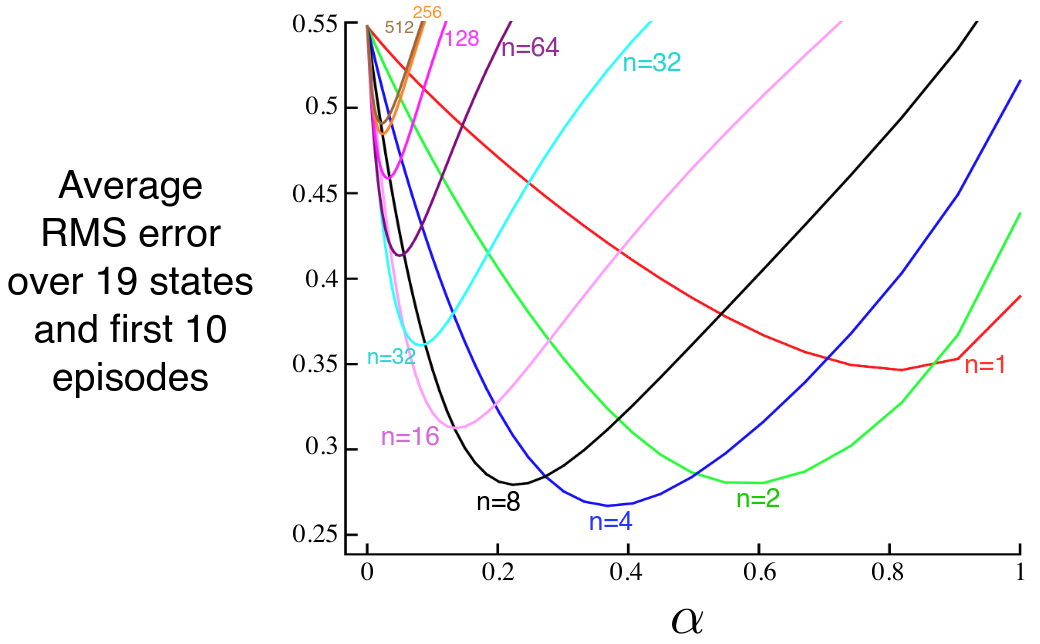
\includegraphics[width=0.8\textwidth]{images/n-step-comparison.png}
    \caption{Comparison between $n$-step methods as a function of $\alpha$ for various values of $n$ in a random-walk task. The $n$-step methods converge faster than both TD methods ($n=1$), and  MC methods ($n=512$).}
    \label{fig:n-step-comparison}
\end{figure}
It can be shown that all $n$-step TD methods converge to the correct value function $v_{\pi}$ under appropriate technical conditions. The $n$-step TD methods hence form a family of sound methods, with one-step TD methods and Monte Carlo methods as extreme members.\\\\
For control problems, we can generalize one-step TD methods to their respective $n$-step versions by defining the $n$-step return in terms of estimated action values.
\begin{equation}
    G_{t:t+n} = R_{t+1} + \gamma R_{t+2} + \dots + \gamma^{n-1} R_{t+n} + \gamma^n Q(S_{t+n}, A_{t+n})
    \label{n-step-return-Sarsa}
\end{equation}
The update rule of $n$-step Sarsa is then the following:
\begin{equation}
    Q(S_t, A_t) = Q(S_t, A_t) + \alpha (G_{t:t+n} - Q(S_t, A_t))
    \label{n-step-action-update}
\end{equation}
In essence, a new TD control algorithm can be constructed by incorporating a formula for the return into Equation \eqref{n-step-action-update}.\\
For example, we can define $n$-step Expected Sarsa by defining the $n$-step return in terms of the expected value of state $S_{t+n}$.
\begin{equation}
    G_{t:t+n} = R_{t+1} + \gamma R_{t+2} + \dots + \gamma^{n-1} R_{t+n} + \gamma^n \sum_a{Q(S_{t+n}, a) \pi(a | S_{t+n})}
    \label{n-step-return-expected-Sarsa}
\end{equation}
And $n$-step Q-learning by defining the $n$-step return in terms of the maximum value of state $S_{t+n}$.
\begin{equation}
    G_{t:t+n} = R_{t+1} + \gamma R_{t+2} + \dots + \gamma^{n-1} R_{t+n} + \gamma^n \max_a{Q(S_{t+n}, a)}
    \label{n-step-return-Q-learning}
\end{equation}

It can be shown that all $n$-step methods converge to the optimal value function if the leaning  and that the convergence rate is independent of $n$.

\section{Discussion}
In this chapter we introduced the main concepts of reinforcement learning, we saw that reinforcement learning is a framework for learning in sequential decision-making problems, where the agent interacts with the environment and learns to maximize its reward.\\
We then presented Monte Carlo methods, which are a class of algorithms that use the full return \eqref{return} to estimate the value function, and TD methods, which use the one-step return \eqref{return-recursive}. TD methods are usually better than MC methods because they can be applied to continuing tasks, and reduce the variance of the value estimate.\\
Finally, we discussed $n$-step methods, which estimate the value function using the $n$-step return formula \eqref{n-step-return}. These methods have been proven to converge to the correct value function $v_{\pi}$ under specific conditions and represent a family of reliable techniques, with one-step TD methods and Monte Carlo methods being their two ends of the spectrum.
